\section{Interpolation / Extrapolation Tool\label{interpolation}}

It is often desirable to predict performance of non-existant machines, or across architectures. This section describes the  tool that rewrites the bgTrace trace logs to provide new sequential execution block durations. These new durations are based upon multiple types of models. The tool can be easily modified to add new types of models if the user requires. The models can be generated from full or partial executions of an application on the target processor or cycle-accurate simulator. 


When predicting the runtime of a parallel application on a not-yet-existent parallel platform, there are two important concerns. The first is correctly modeling the interconnection network which is handled by BigSimulator (also called BigNetSim). The second is determining the durations of the relevant sequential portions of code, which we call \textbf{Sequential Execution Blocks (SEB)}, on a new type of processor. The interpolation tool of this section handles only the prediction of durations of SEBs using 3 types of currently implemented models:

\begin{enumerate}
\item \textbf{Scale SEB durations} recorded on an available processor by a constant factor $s$.
\item \textbf{Parameterizations} of SEBs. Each SEB is augmented with user defined parameters which influence the duration of the SEB. A model based on the parameters can extrapolate to SEBs not instrumented in the initial emulation run.
\item \textbf{Parameterizations with cycle-accurate simulations} for non-existant architectures. Processor designers use cycle-accurate simulators to simulate the performance of a piece of code on a future processor which is currently unavailable.  Timings for each SEB can be performed in such a cycle-accurate simulator. The cycle-accurate timings can be extrapolated to SEBs not instrumented in the cycle-accurate simulator.
\end{enumerate}

Soon the tool will also support performance counters in a new model.

The interpolation tool rewrites the log files produced by a run in BigEmulator. The rewritten log files will then be consumed by BigSimulator. This flow can be seen in figure \ref{fig:interpolationflow}. Multiple types of models are supported in the tool. 

\begin{figure}[!t]
\centering  
  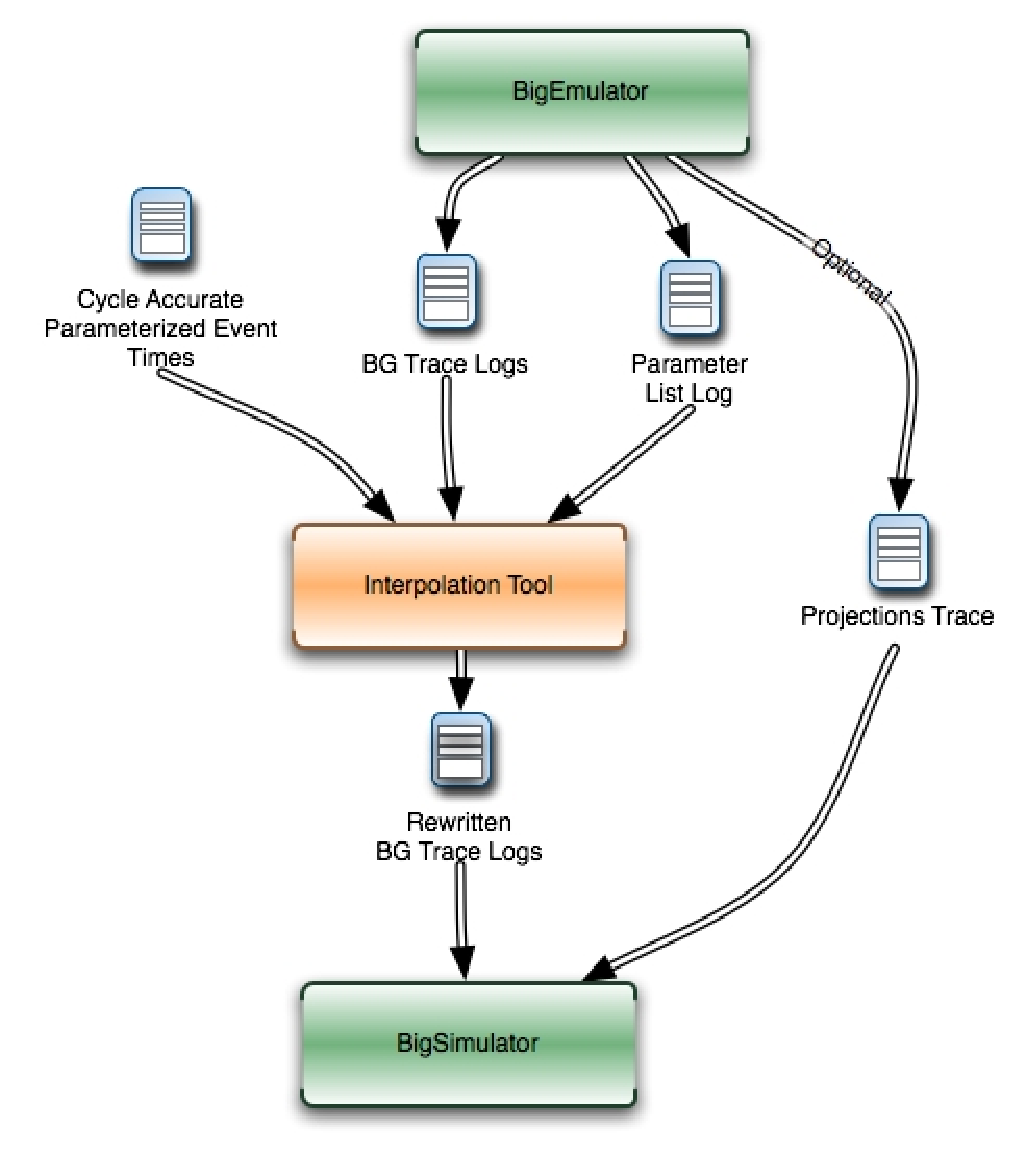
\includegraphics[width=4in]{figures/InterpolationFlow}
{\sffamily\bfseries\small \caption{Flow diagram for interpolation tool\label{fig:interpolationflow}}}
\end{figure}

%%%%%%%%%%%%%%%%%%%%%%%%%%%%%%%%%%%%%%%%%%%%%%%%%%%%
\subsection{Usage\label{usage}}

The interpolation tool can be found in the directory \texttt{charm/examples/bigsim/tools/rewritelog} with a \texttt{README} file describing its use in more detail than this manual.

\subsubsection{Producing the Parameterized Timings Log}
The interpolation tool uses as input a log of actual runtimes of user-bracketed sequential execution blocks. These timings come from a full or partial execution of the parallel application on a real machine or within a cycle-accurate simulator. 

The user must insert \texttt{startTraceBigSim()} and  \texttt{endTraceBigSim()} calls around the main computational regions in the parallel application. These two calls time the region between them and print out a record for each compuatational region. The functions should be called at most once during any SEB. The output from  \texttt{endTraceBigSim()} is a line similar to ``\texttt{TRACEBIGSIM: event:\{ PairCalculator::bwMultiplyHelper \}  time:\{ 0.002586 \}  params:\{ 16384.00 1.00 220.00 128.00 128.00 0.00 0.00 0.00 \}}.'' The event name and up to 20 parameters are specified in the call to  \texttt{endTraceBigSim()} and the \texttt{time} field records  the duration of the bracketed region of sequential code. 

To run in a cycle-accurate simulator such as IBM's MAMBO, the  \texttt{startTraceBigSim()} and  \texttt{endTraceBigSim()} functions would be modified to switch between the fast forward mode used during the rest of the program and the cycle-accurate mode during the bracketed region of code. The functions are provided in C++ source files in the directory \texttt{charm/examples/bigsim/tools/rewritelog/traceBigSim} which must be added to an application manually.

%%%%%%%%%%%%%%%%%%%%%%%%%%%%%%%%%%%%%%%%%%%%%%%%%%%%
\subsubsection{The bgTrace log file format}

The bgTrace log has data from emulation of the full parallel application with an entry for each SEB with the following fields:  \textit{ID}, \textit{Name}, $T_{start}$, $T_{end}$, \textit{Back}, \textit{Forward}, \textit{Message ID}, \textit{Source Node}, \textit{Message ID}, \textit{Sent Messages}. The final field is actually a list of records for each message sent by the entry method. Each record contains the following fields:  \textit{Message ID}, $T_{sent}$, $T_{recv}$, \textit{Destination PE}, \textit{Size}, \textit{Group}.

The interpolation tool will rewrite the durations of the events by correcting the $T_{end}$ field for the event and the $T_{sent}$ fields for each send message. The new durations of all SEBs will be based upon some model $M:SEB\rightarrow Duration$. 

Each SEB is composed of three temporal regions as shown in figure \ref{event_diagram}. The entire SEB is associated with a Charm++ entry method, while the middle region is the computational kernel bracketed by the user's \texttt{startTraceBigSim()} and  \texttt{endTraceBigSim()} calls. The model is used only to approximate the new duration of the middle temporal region. The duration of the beginning and end region are scaled by a simple constant factor.

\begin{figure}
\centering
\includegraphics[width=5in]{figures/event_diagram}
\caption{SEBs in the bgTrace file have a start and end time. Only a portion of the SEB, e.g. the important compuational kernel, is timed when performing cycle accurate simulation. The duration of the middle portion of the SEB can be estimated in a different manner than the rest of the SEB. For example, the begin and end pieces can be scaled by some constant factor, while the bracketed middle region's duration is estimated based on a model\label{event_diagram}}
\end{figure}

The interpolation tool internally take the ID for each SEB and looks up its associated parameters. If parameters are found, they are used as input to $f$ to evaluate the new duration $d_{new}$ for the SEB. The end time is then modified to be $T_{end}\leftarrow  T_{start}+d_{new}$.

\begin{figure}
\centering
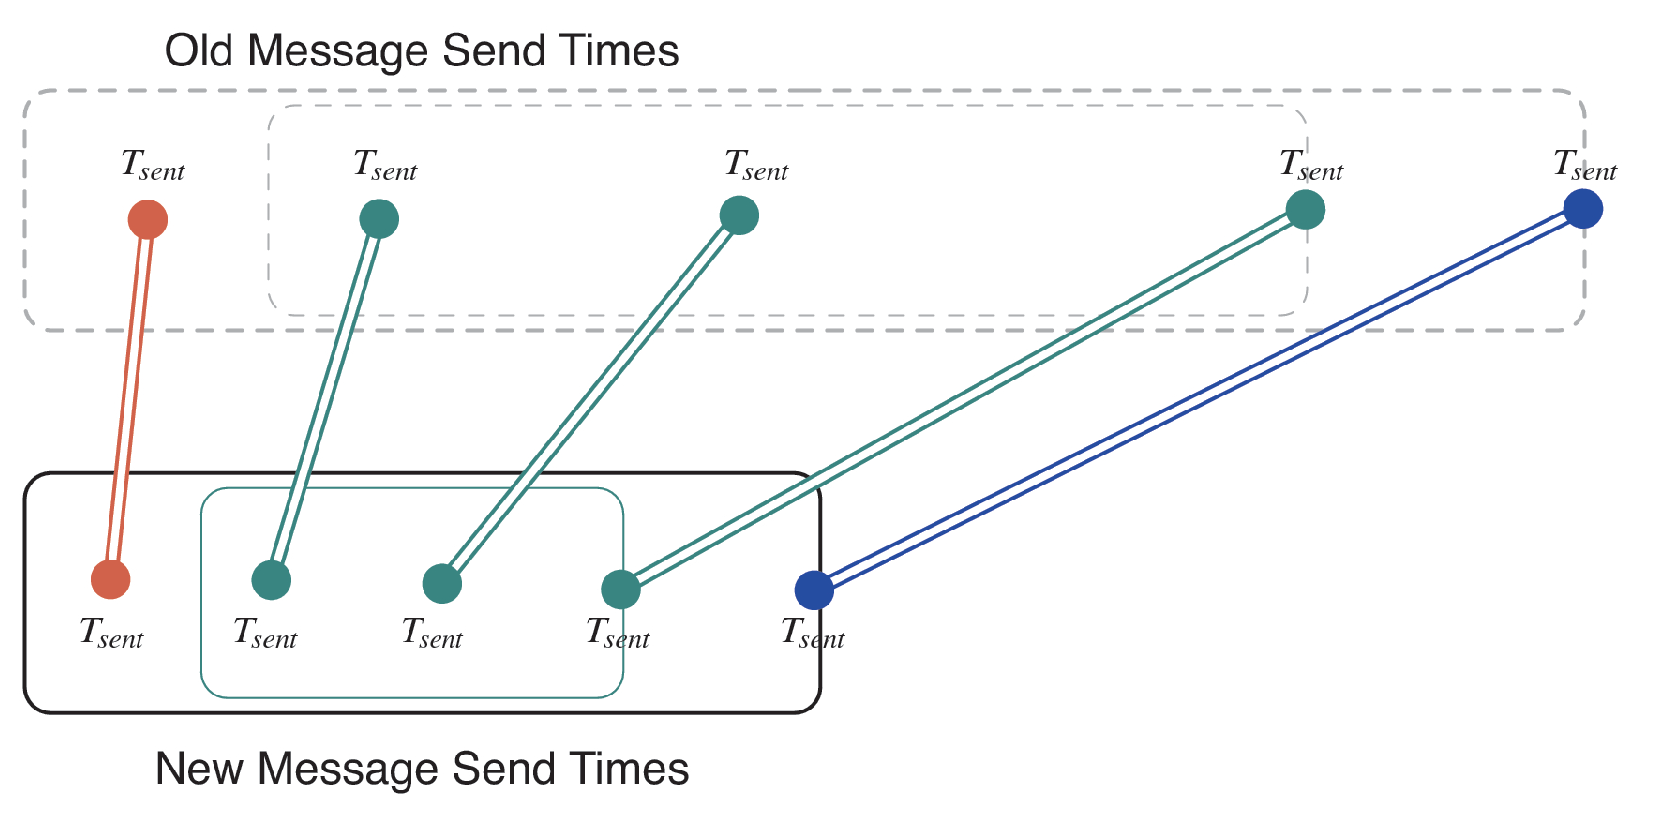
\includegraphics[width=6in]{figures/event_diagram2}
\caption{Message send times for messages sent from an SEB are remapped linearly onto the new time ranges for the SEBs, region by region\label{event_diagram2}}
\end{figure}

The messages in the message list for each SEB must also have their $T_{sent}$ times rewritten. This is accomplished by linearly mapping the old $T_{sent}$ value from to the new range for the enclosing SEB region, as shown in Figure \ref{event_diagram2}. Any message sent during the first portion will be mapped linearly onto the new first portion of the SEB. The new message $T_{recv}$ times are ignored by BigSimulator, so they do not need to be modified.


\subsubsection{Supported performance models}
The interpolation tool supports three types of models described in sections \ref{sec:model:scale}, \ref{sec:model:parameterization}, and \ref{sec:model:partial}. 

The more complicated models use the least-square curve fitting technique. The current implementation uses the Gnu Scientific Library(gsl) to perform the least-square fit to the given data. The library provides both the coefficients and a $\chi^2$ measure of the closeness of the fit to the input data. 


%%%%%%%%%%%%%%%%%%%%%%%%%%%%%%%%%%%%%%%%%%%%%%%%%%%%
\subsubsection{Model 1: Scaling SEB durations from a full run on target processor\label{sec:model:scale}}

In simple cases, a sufficient approximation of the performance of a parallel application can be performed by simply multiplying the SEB durations by a constant factor.  A user may know a desired target machine has processors that will execute each SEB twice as fast as on an existing machine. The application is emulated on the existing machine, and the SEB durations are scaled by a factor of $2.0$. This method is simple, but may be sufficient in many cases. In this case it is unnecessary to use the \texttt{startTraceBigSim()} and  \texttt{endTraceBigSim()} calls. The scaling factor is hard coded in the interpolation tool as \texttt{time\_dilation\_factor}. It is used to scale all events unless a suitable advanced model has a better method for approximating the duration. It will always be used to scale any portions of events that are not bracketed with the calls \texttt{startTraceBigSim()} and  \texttt{endTraceBigSim()}.

\subsubsection{Model 2: Extrapolating based on User Parameterizations\label{sec:model:parameterization}}

The user can simply insert the bracketing calls  \texttt{startTraceBigSim()} and  \texttt{endTraceBigSim()} around the computational kernels to log the times taken for each. Unfortunately, the duration of the SEB will likely depend upon the data distribution and access patterns for the parallel application. Thus the user will specify parameters likely to influence the SEB duration. The parameters will include variables indicating number of loop iterations, number of calls to computational kernels, or sizes of accessed portions of data arrays. A model is built to approximate the duration of any SEB based upon its specified parameters.

For example, NAMD uses a number of different types of objects. The \texttt{compute} objects will spend varying amounts of time depending upon the lengths of their associated atom lists. If an atom list is large, more interactions are computed and thus more computation is performed. 

Now the method is described in the context of a simple hypothetical molecular dynamics application. Assume the Charm++ entry method called \texttt{doWork(atomList)} is where a majority of the work from the application occurs. The function computes forces on atoms of various types. Different calls to the function will contain different numbers and types of attoms. The source for  \texttt{doWork(atomList)} will be modified by the user to  contain calls to  \texttt{startTraceBigSim()} at the beginning and  \texttt{endTraceBigSim()} at the end of the function. The program will be run, and the resulting timed samples will be used to build a model. Assume the expected runtime of \texttt{doWork(atomList)} is quadratic in the \texttt{atomList} length and linear in the number of carbon atoms in the \texttt{atomList}. The \texttt{endTraceBigSim()}  call will be provided with a descriptive name and a set of parameters: \texttt{endTraceBigSim(``doWork()'', $p_1$,$p_2$)}  where parameter $p_1$ is the length of \texttt{atomList} and parameter $p_2$ is the number of carbon atoms in \texttt{atomList}.

The goal is to be able to predict the execution time of any arbitrary call to \texttt{doWork()} given its parameters. The molecular dynamics application is run on an existing processor or parallel cluster for only a few timesteps with the modified \texttt{doWork()} method. This run will produce a list of $\left(p_1,p_2\right)\rightarrow duration$ records. A least squares method is applied to fit a curve $f(p_1,p_2)=c_1+c_2 p_1+c_3 p_1^2 + c_4 p_2$  approximating the durations to the records. The least squares method minimizes the sum of the squares of the difference between the function $f$ evaluated at each parameter set and the actual timing at those parameters. The least square method is provided  $\left(1.0,p_1,p_1^2,p_2,time\right)$ for each sample point and it produces the coefficients $c_n$ in $f$. An arbitrary set of parameters can be input to $f$ to produce an approximation of the runtime of \texttt{doWork()} even though the particular instance was never timed before. 

\subsubsection{Model 3: Extrapolating Partial Executions with Cycle Accurate Simulations and User Parameterizations\label{sec:model:partial}}

In this case, a cycle accurate simulator can be used to time a small fraction of all SEBs for a run of the application. The partial execution is used to build a model which applies to the whole execution. Parameterizations can be used as in section \ref{sec:model:parameterization} so that only some fraction of the SEBs will be run in the expensive cycle-accurate simulator. For example, in NAMD, a sufficient model can be build from  a random sample of 2\% of the cycle-accurate SEB durations from 4 timeloop iterations. 
